\documentclass[main]{subfiles}

\begin{document}


\chapter{Pruebas sobre el controlador}
\label{chap:test_control}

El objetivo de la presente secci\'on es el de analizar el desempeño del controlador. Nos concentraremos entonces en analizar algunos par\'ametros fundamentales del mismo, es de particular inter\'es conocer la respuesta al escal\'on del sistema para los tres tipos de trayectoria definidos. Modificando la altura del escal\'on se puede determinar la aceleraci\'on m\'axima a la cual podemos someter al sistema en cada trayectoria, esto resulta fundamental a la hora de imponer restricciones sobre la ruta que se desea seguir. Se analizar\'a adem\'as la robustez del controlador implementado, para esto se añade un ruido a los estados realimentados, dicho ruido intenta representar el ruido asociado a las medidas de los sensores. El simulador desarrollado nos permite agregar a cada estado un ruido que cumple con el siguiente modelo:

\begin{equation}
\label{eq:noise}
\eta_i = A_i\cos(\omega t)+\varepsilon(\mu_i,\sigma_i)
\end{equation}

Donde $\varepsilon(\mu_i,\sigma_i)$ es un ruido gaussiano de media $\mu_i$ y de desviaci\'on est\'andar $\sigma_i$.

\section{Respuesta al escal\'on}
Nos centraremos en estudiar las respuestas al escal\'on de los tres tipos de trayectorias. En esta secci\'on no se consideran medidas con ruido, es decir que se conoce el estado a la perfecci\'on.  

\subsection{Trayectoria de hovering}

\subsubsection{Desplazamientos en la direcci\'on vertical}
Se consideran condiciones iniciales nulas. Se fija como setpoint:
\begin{itemize}
\item Prueba 1: ${x_s = 0 m;\quad y_s = 0 m;\quad z_s = 1 m;\quad \theta = 0_s^\circ}$
\item Prueba 2: ${x_s = 0 m;\quad y_s = 0 m;\quad z_s = 100 m;\quad \theta = 0_s^\circ}$
\end{itemize}

No se aprecian variaciones en ninguna de las variables de estado excepto en la posici\'on vertical ($z$) y en la velocidad $v_{q_z}$. Este resultado es perfectamente esperable ya que todas las variables excepto $z$ son iguales al setpoint inicialmente. Para modificar la altura es necesario modificar la velocidad $v_{q_z}$, lo cual explica su variaci\'on. La respuesta al escal\'on para las pruebas uno y dos se muestran en la figura \ref{fig:hov_esc_z}. 
\begin{figure}
  \centering
  \subfloat[Escal\'on de altura 1 m]{\label{fig:Z_1}
  		\includegraphics[width=0.5\textwidth]
  			{./pics_test_control/step_hov_z_1.pdf}}
  \subfloat[Escal\'on de altura 100 m]{\label{fig:z_100}
  		\includegraphics[width=0.5\textwidth]
  			{./pics_test_control/step_hov_z_100.pdf}}
  \caption{Respuesta al escal\'on en la altura}
  \label{fig:hov_esc_z}
\end{figure}

Tanto el tiempo de \emph{rise} como el sobretiro presentado por la respuesta al escal\'on son considerados ampliamente satisfactorios. Para la primera prueba se obtiene un tiempo de \emph{rise} de $2.26 s$ y no hay sobretiro. Para el escal\'on de $100m $ el tiempo de \emph{rise} es de $5.06 s$. En esta prueba aparece un sobretiro inferior a los dos metros. \\

Los resultados obtenidos en la simulaci\'on son ampliamente satisfactorios ya que nos indican que se puede aclanzar un rango de alturas muy amplio en pocos segundos sin que el sistema presente comportamientos que impliquen inestabilidad. Por otra parte se observa en ambas pruebas que una vez alcanzado el valor objetivo se mantiene perfectamente.\\

\begin{figure}
  \centering
  \subfloat[Velocidad en la direcci\'on vertical]{\label{fig:vqz_100}
  		\includegraphics[width=0.5\textwidth]
  			{./pics_test_control/vqz_100.pdf}}
  \subfloat[Velocidad angular del motor 1]{\label{fig:z_100_w}
  		\includegraphics[width=0.5\textwidth]
  			{./pics_test_control/z_100_w.pdf}}
  \caption{Respuestas de la velocidad vertical y la velocidad angular de los motores para el escal\'on de 100m}
  \label{fig:hov_esc_z_otros}
\end{figure}

Si estudiamos la velocidad vertical del sistema en la segunda prueba nos encontramos con que se alcanza la velocidad m\'axima ( $22.05 ms^{-1}$ ) en $6.46 s$. Lo cual implica una aceleraci\'on de $3.41 ms^{-2}$. Por otra parte, luego de alcanzada la velocidad m\'axima esta comienza a disminuir, la aceleraci\'on el tramo en cuesti\'on es de $-7.09ms^{-2}$. Estas aceleraciones son  la m\'axima y m\'inima posible en la direcci\'on vertical ya que, como puede observarse en la figura \ref{fig:z_100_w} la velocidad angular de los motores satura, llegando tanto a su velocidad m\'axima y m\'inima. 

\subsubsection{Desplazamientos en la direcci\'on horizontal}
Partiendo de condiciones iniciales nulas excepto la altura donde se considera $z = 3 m$, se fija el siguiente setpoint:
\begin{itemize}
\item ${x_s = 5 m;\quad y_s = 0 m;\quad z_s = 3 m;\quad \theta = 0_s^\circ}$
\end{itemize}

En la figura \ref{fig:step_x} se observa la trayectoria del sistema solidario al cuadric\'optero a lo largo del tiempo. El comportamiento es acorde a lo esperado. Se observa que el cuadric\'optero tiende a descender inicialmente para luego recuperar su posici\'on inicial. Esto se debe a que en el instante en el cual se produce el escal\'on en el setpoint, se tiene que $z-z_s = 0$, por lo tanto, los t\'erminos de K que dependen de las diferencias no se hacen presentes en la realimentaci\'on, a diferencia de lo que sucede con los t\'erminos que dependen de $x-x_s$.  Todo sucede como si inicialmente el controlador no controlara la altura. En la figura \ref{fig:step_hov_x_z} puede apreciarse que la variaci\'on de la altura es cercana a los $0.3 m$. Se realizaron simulaciones para valores de $x_s > 5 m$, pero los resultados en cuanto a la variaci\'on de las restantes variables de estado no fueron considerados satisfactorios. Por otra parte la aceleraci\'on m\'axima a la cual deber\'ia ser sometido el cuadric\'optero en la direcci\'on horzontal debes ser menor a los $2 ms^{-2}$. Estos \'ultimos aspectos no implican que el control para la condici\'on de hovering sea defectuoso, el controlador fue diseñado linealizando en torno a una trayectoria en la cual $\vec{V} = 0$, por lo tanto es razonable suponer que para no sea adecuado para controlar desplazamientos importantes. En el caso del eje $z$ se obtuvo un desplazamiento importante ya que solamente es necesario modificar la variable $v_{q_z}$ la cual, al tener $\vec{\omega} = 0$ no implica variaciones en ninguna otra variable de estado. Para realizar un desplazamiento seg\'un la direcci\'on horizontal deben modificarse o bien el \'angulo de Roll o bien el \'angulo de Pitch. Sucede que tanto, las velocidades como las posiciones dependen de dichos \'angulos, por lo tanto variaciones importantes en los mismos nos alejan de la condici\'on para la cual se linealiz\'o el sistema.\\

En res\'umen, se desarroll\'o un controlador que nos permite grandes desplazamientos en la direcci\'on vertical $(\approx 100m )$ y desplazamientos inferiores a los $5 m$ en la horizontal, con tiempos de respuesta inferiores a los $5.06 s$ y $2.16 s $ respectivamente, al menos sin presencia de ruido de medici\'on.  

\begin{figure}
  \centering
  \subfloat[Ejes solidarios al cuadric\'optero a lo largo del tiempo]{\label{fig:step_x}
  		\includegraphics[width=0.35\textwidth]
  			{./pics_test_control/step_x.pdf}}
  \subfloat[Posici\'on seg\'un $\vec{i}_I$]{\label{fig:step_hov_x_5}
  		\includegraphics[width=0.35\textwidth]
  			{./pics_test_control/step_hov_x_5.pdf}}
  \subfloat[Altura en m]{\label{fig:step_hov_x_z}
  		\includegraphics[width=0.35\textwidth]
  			{./pics_test_control/step_hov_x_z.pdf}}
 
  \caption{Escal\'on de 2m en la direcci\'on horizontal}
  \label{fig:hov_esc_x}
\end{figure}

\section{Robustez frente a la presencia de ruido de medici\'on}

Hasta aqu\'i hemos evaluado las caracter\'isticas del controlador diseñado en situaciones en las cuales se conoce exactamente el vector de estados, evidentemente la situaci\'on de vuelo real no se corresponde con esta idealidad. Las medidas realizadas tienen ruido intr\'inseco, muy superior a los considerados en las pruebas de calibraci\'on y caracterizaci\'on de los sensores. El aumento de este ruido se debe principalmente a las vibraciones mec\'anicas que introducen las h\'elices.\\

Resulta fundamental conocer en forma aproximada el comportamiento de los ruidos de medida. Con dicho fin se realiz\'o una prueba de vuelo en la cual el cuadric\'optero estaba sujeto por arriba y por debajo quedando imposibilitado de realizar movimientos. Se comandaron los motores a la velocidad de hovering. En la presente secci\'on se presentan los par\'ametros de la ecuaci\'on \ref{eq:noise} que mejor ajustan el ruido. Si bien se podr\'ia haber realizado dicho ajuste utilizando m\'inimos cuadrados, al menos para la parte del ruido no aleatorio, se opt\'o por realizar dicho ajuste en forma iterativa.\\

Dado que los \'angulos de pitch y de roll se obtienen directamente con los aceler\'ometros los ruidos asociados a ambas medidas son id\'enticas. Por dicho motivo consideraremos un solo ruido replicado en ambas variables. En el caso de las velocidades angulares y de la posici\'on horizontal (medida con el GPS), trabajaremos de la misma forma.\\ 

Finalmente cabe aclarar que se espera que los ruidos obtenidos sean independientes del tipo de trayectoria realizada, por lo tanto los ruidos obtenidos para la trayectoria de hovering ser\'an los utilizados para las restantes. 
\subsection{Hovering}

Para el ruido asociado a las medidas de los \'angulos de pitch y de roll se escogieron los siguientes par\'ametros:

\begin{itemize}
\item $A_{roll} = 0.05^\circ$
\item $\omega_{i_{roll}} = 2\pi 0.03 rads^{-1}$
\item $\sigma_{roll} = 6.05^\circ$
\item $\mu_{roll} = 0.27 ^\circ$
\end{itemize}
  
En la figura \ref{fig:ruido_roll} pueden compararse los ruidos obtendidos en la ``situaci\'on de vuelo'' descripta anteriormente y el ruido en la simulaci\'on. Asimismo puede observarse como, a pesar de la gran presencia de ruido la variable de estado de inter\'es se mantiene controlada muy cercana al valor deseado. El valor m\'aximo y m\'inimo de roll alcanzados son $6.48^\circ$ y $-6.41^\circ$.\\

En la figura \ref{fig:roll_vuelo} se observan tres amplitudes de ruido bien marcadas. La primera corresponde a las medidas con los motores apagados, la segunda a partir del segundo 20.5 donde los motores operan a velocidad m\'inima ($109 rev s^{-1}$) y la tercera a partir del segundo 34 donde la velocidad angular de los motores es igual a la velocidad de hovering. En lo que sigue del an\'alisis nos concentraremos exclusivamente en esta tercer etapa.\\

\begin{figure}
  \centering
  \subfloat[Medida del \'angulo de Roll en ``situaci\'on de vuelo'']{\label{fig:roll_vuelo}
  		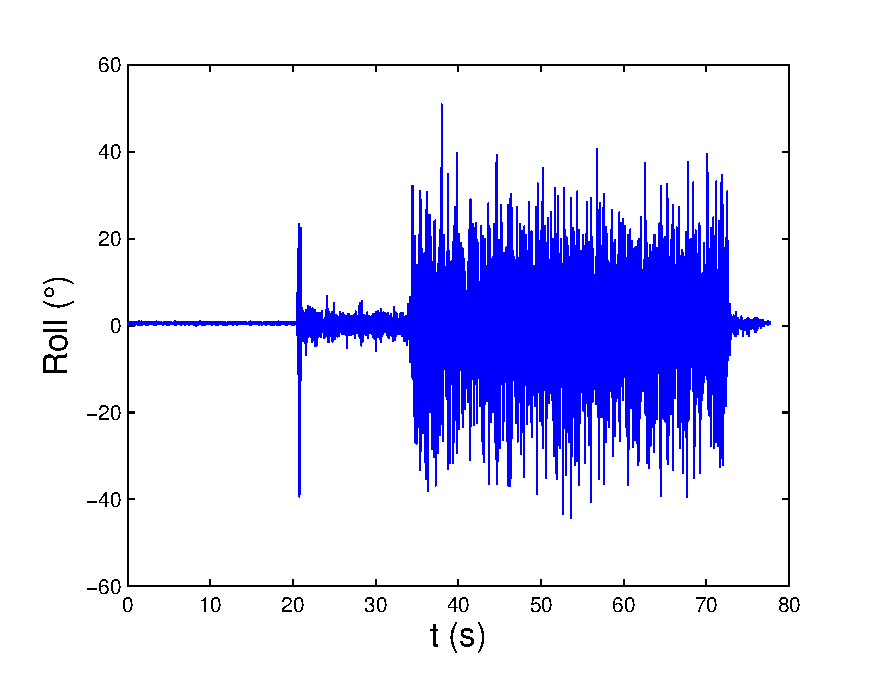
\includegraphics[width=0.5\textwidth]
  			{./pics_test_control/ruido/roll_vuelo.pdf}}
  \subfloat[Ruido de Roll simulado y Roll efectivo ]{\label{fig:roll_noise}
  		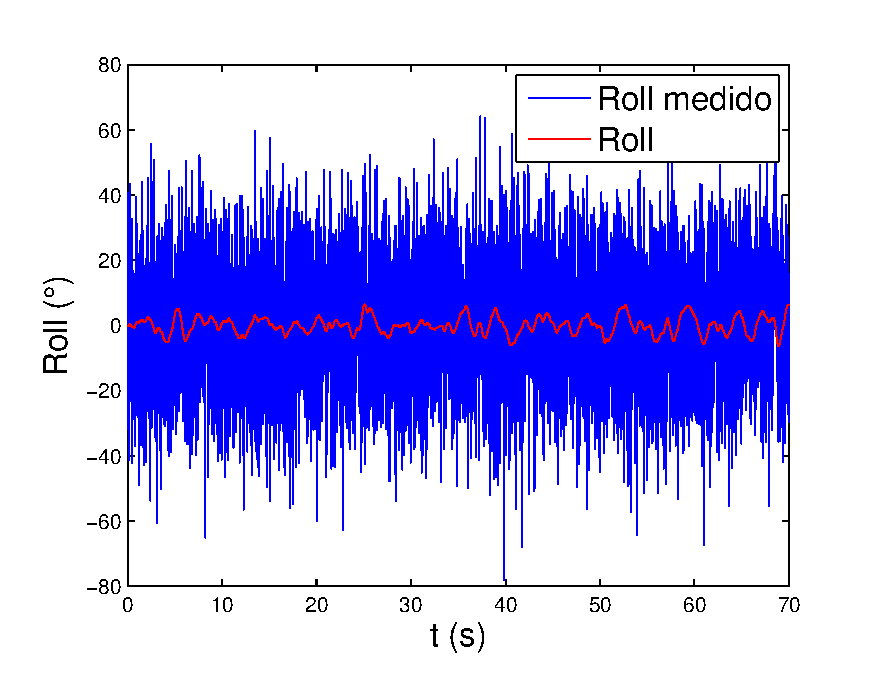
\includegraphics[width=0.5\textwidth]
  			{./pics_test_control/ruido/roll_noise.pdf}}
  \caption{Ruidos de Roll}
  \label{fig:ruidos_roll}
\end{figure}
  
El \'angulo de Yaw se determina adem\'as utilizando la lectura del magnet\'ometro, por dicho motivo se separa el an\'alisis de su ruido de los restantes \'angulos de Euler. En este caso los par\'ametros de ruido utilizados son:

\begin{itemize}
\item $A_{yaw} = 0.23^\circ$
\item $\omega_{yaw} = 2\pi 0.07 rad s^{-1}$
\item $\sigma_{yaw} = 2\circ$
\item $\mu_{yaw} = 0$
\end{itemize}

En la figura \ref{fig:ruidos_yaw} puede observarse como, a pesar del ruido en la medida el controlador se mantiene robusto apart\'ndose del valor objetivo $0.96^\circ$ en el peor de los casos. El resultado en lo que respecta al control de la velocidad angular del sistema es similar. En la figura \ref{fig:ruidos_wqx} pueden observarse las gr\'aficas de los ruidos medido y simulado, adem\'as de la velocidad angular ``real''. Se trabaja en este caso con la velocidad angular $\omega_{q_x}$. Los par\'ametros de ruido escogidos son:
\begin{itemize}
\item $A_{\omega_{q_x}} = 0.03^\circ s^{-1}$
\item $\omega_{\omega_{q_x}} = 2\pi 0.03 rad s^{-1}$
\item $\sigma_{\omega_{q_x}} = 0.64\circ s^{-1}$
\item $\mu_{\omega_{q_x}} = 0$
\end{itemize}
\begin{figure}
  \centering
  \subfloat[Medida del \'angulo de Yaw en ``situaci\'on de vuelo'']{\label{fig:yaw_vuelo}
  		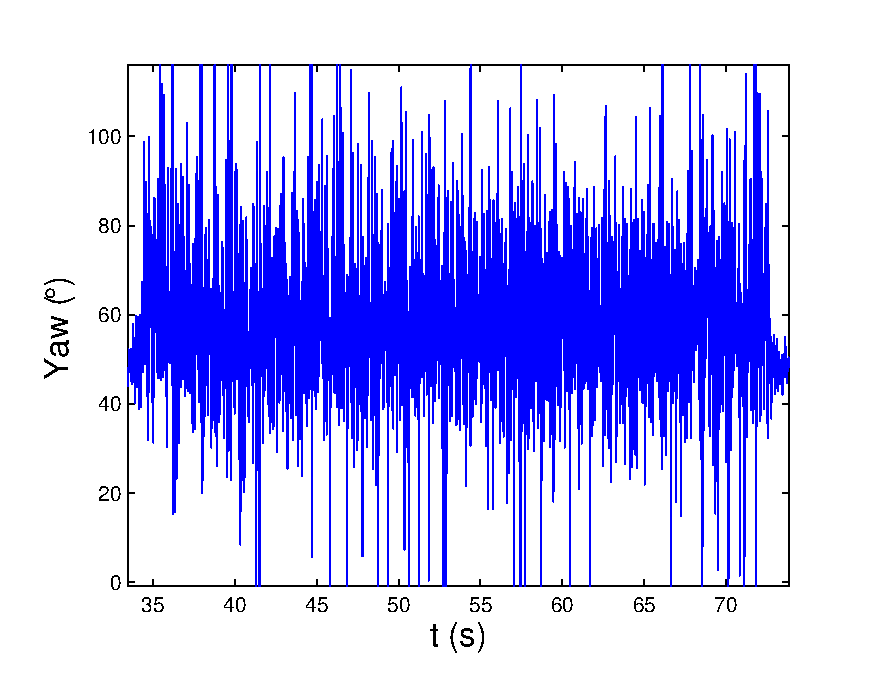
\includegraphics[width=0.5\textwidth]
  			{./pics_test_control/ruido/yaw_vuelo.pdf}}
  \subfloat[Ruido de Yaw simulado y Yaw efectivo ]{\label{fig:yaw_noise}
  		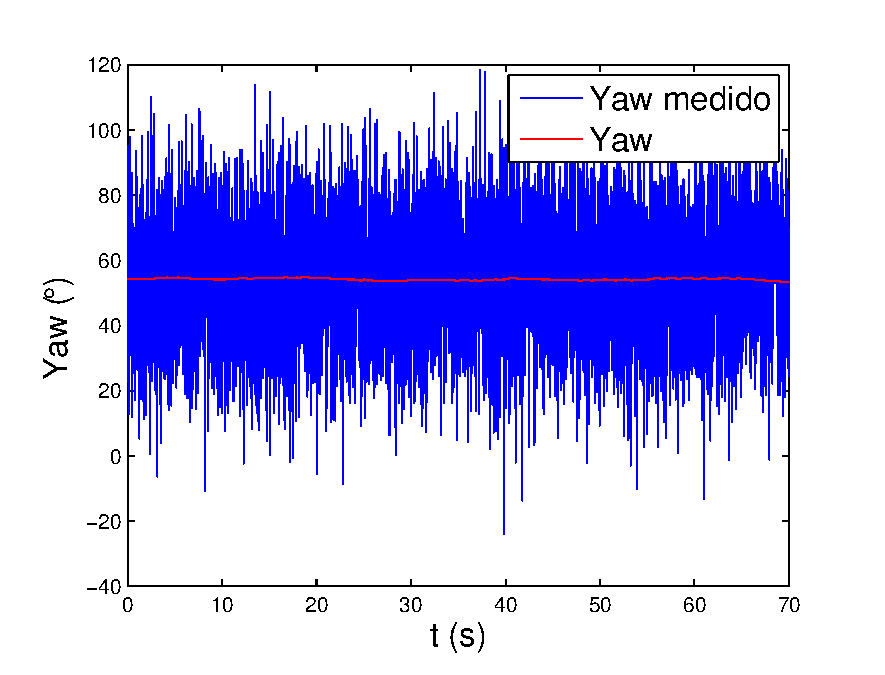
\includegraphics[width=0.5\textwidth]
  			{./pics_test_control/ruido/yaw_noise.pdf}}
  \caption{Ruidos de Yaw}
  \label{fig:ruidos_yaw}
\end{figure}


\begin{figure}
  \centering
  \subfloat[Medida de $\omega_{q_x}$ en ``situaci\'on de vuelo'']{\label{fig:wqx_vuelo}
  		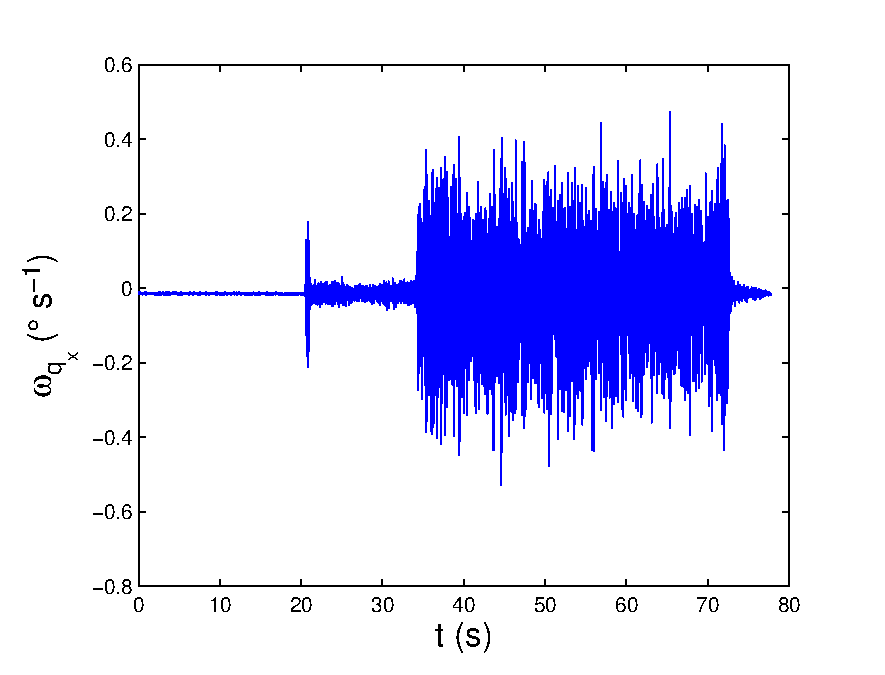
\includegraphics[width=0.5\textwidth]
  			{./pics_test_control/ruido/wqx_vuelo.pdf}}
  \subfloat[Ruido de $\omega_{q_x}$ simulado y $\omega_{q_x}$ efectivo ]{\label{fig:wqx_noise}
  		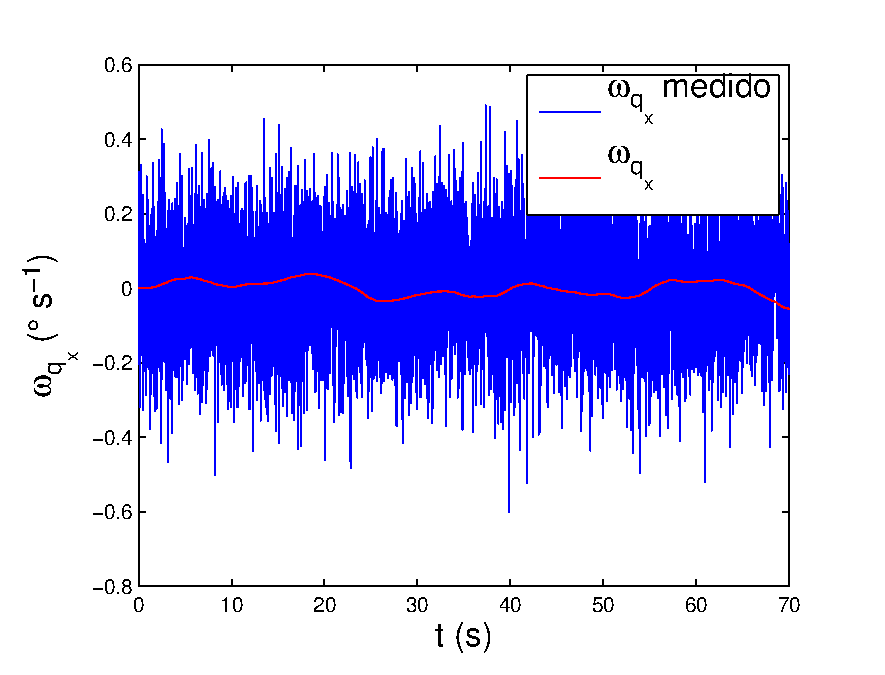
\includegraphics[width=0.5\textwidth]
  			{./pics_test_control/ruido/wqx_noise.pdf}}
  \caption{Ruidos de $\omega_{q_x}$}
  \label{fig:ruidos_wqx}
\end{figure}


Los ruidos observados hasta el momento son preponderamente blancos. Por dicho motivo es practicamente imposible observar la respuesta del control m\'as all\'a de afirmar que efectivamente no nos alejamos sustancialmente de la posici\'on deseada. En el caso del ruido en la altura la situaci\'on es distinta ya que quien juega el papel m\'as importante en el ruido es una oscilaci\'on de baja frecuencia. Los par\'ametros elegidos para representar dicho ruido son:

\begin{itemize}
\item $A_z = 1 m$
\item $\omega_{z} = 2\pi 0.04 rad s^{-1}$
\item $\sigma_{z} = 0.34 m$
\item $\mu_{z} = 0.94 m$
\end{itemize}

\begin{figure}
  \centering
  \subfloat[Medida de z en ``situaci\'on de vuelo'']{\label{fig:z_vuelo}
  		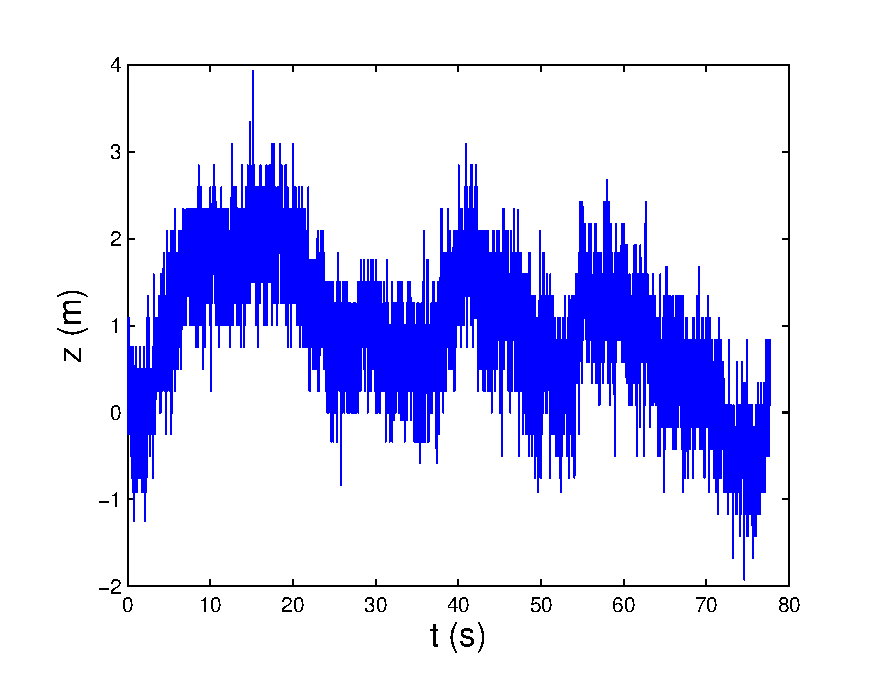
\includegraphics[width=0.5\textwidth]
  			{./pics_test_control/ruido/z_vuelo.pdf}}
  \subfloat[Ruido de z simulado y z efectivo ]{\label{fig:z_noise}
  		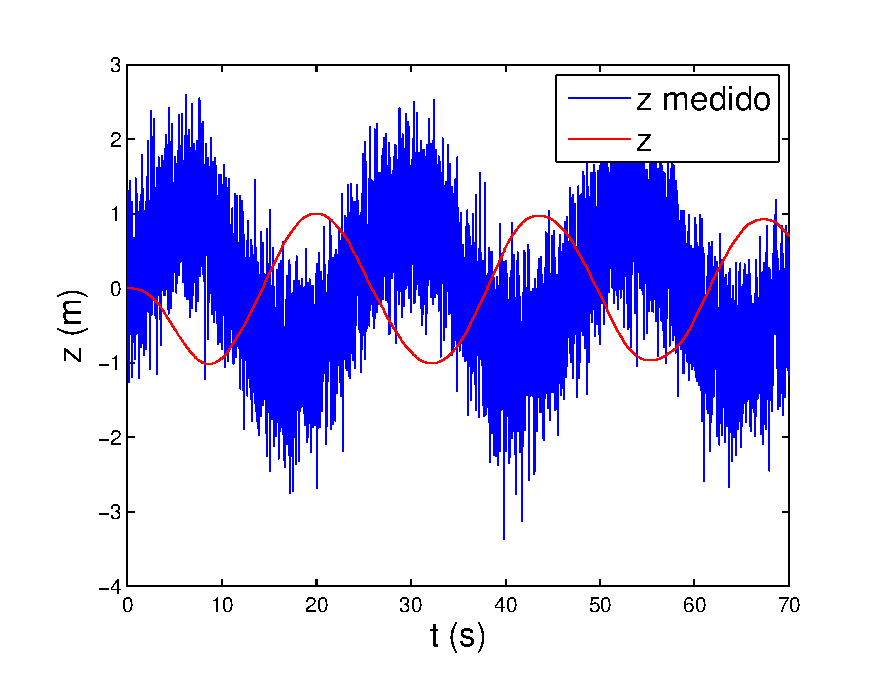
\includegraphics[width=0.5\textwidth]
  			{./pics_test_control/ruido/z_noise.pdf}}
  \caption{Ruidos de z}
  \label{fig:ruidos_z}
\end{figure}

En la figura \ref{fig:z_noise} se aprecia claramente la acci\'on del control ya que para medidas que superan el valor deseado de \emph{setpoint} el control act\'ua en sentido contrario, sucede lo mismo para las medidas que son inferiores al \emph{setpoint}.

Los ruidos que se han menejado hasta aqu\'i corresponden a las medidas directa de los sensores. Al someter estas medidas al filtro de Kalman (ver cap\'itulo \ref{chap:kalman}) tendremos ruidos muy inferiores. Por lo tanto podemos asumir que el sistema se comportar\'a a\'un mejor que lo que se evalu\'o en esta secci\'on.\\

En lo que respecta al ruido de la velocidad no se puede trabajar simplemente con las medidas de los sensores ya que no se tiene ninguna medida directa de la velocidad. La \'unica medida que se tiene es la aceleraci\'on, se podr\'ia integrar dicha medida para obtener valores de velocidad, pero el error introducido en la aceleraci\'on lleva a que la velocidad tenga una deriva, no tiene sentido en pensar esta magnitud con un ruido asociado, excepto que trabajemos en este caso con las estimaciones del vector de estados. 



\end{document}